\documentclass{beamer} %
\usetheme{Dresden}
\usecolortheme{beaver}
\usepackage[portuguese]{babel}
\usepackage[utf8x]{inputenc}
\usefonttheme{professionalfonts}
\usepackage{times}
\usepackage{tikz}
\usepackage{amsmath}
\usepackage{tabulary}
\usepackage{pgfgantt}
\usepackage{verbatim}
\usetikzlibrary{arrows,shapes}
\usepackage{adjustbox}
\usepackage{soul}
\usepackage{listings}
\usepackage{adjustbox}
\setbeamertemplate{itemize item}{\color{red}$\blacksquare$}
\usepackage{hyperref}
\title{avance1}
\bibliographystyle{plainnat}


\newtheorem{defi}{Definição}
\newtheorem{lema}{Lema}
\newtheorem{teo}{Teorema}
\newtheorem{prop}{Proposição}
\newtheorem{prova}{Demonstração}
\newtheorem{exemplo}{Exemplo}
\newtheorem{hipotese}{Hipótese}
\newtheorem{algo}{Algoritmo}
\newcommand{\R}{\mathbb{R}}
%\newcommand{\P}{\mathcal{P}}
\newcommand{\C}{\mathcal{C}}
\newcommand{\I}{\mathcal{I}}
\newcommand{\A}{\mathcal{A}}
\newcommand{\F}{\mathcal{F}}
\newcommand{\X}{\mathcal{X}}
\newcommand{\Y}{\mathcal{Y}}
\newcommand{\M}{\mathcal{M}}
\newcommand{\E}{\mathbb{E}}
\newcommand{\V}{\mathbb{V}}
\newcommand{\Prob}{\mathbb{P}}
\newcommand{\Tau}{\mathrm{T}}
\newcommand{\1}{\mathbb{I}}


\title{Computação de Efeitos Marginais em Florestas Aleatórias}
\institute[]{Universidade Federal Fluminense}
\author{Pedro Cavalcante Oliveira}

\date{\today}

\begin{document}
\tikzstyle{every picture}+=[remember picture]
\lstset{language=C++}   
\everymath{\displaystyle}

\begin{frame}

	\titlepage
\end{frame}

%------------------------------------------------------


\begin{frame}

Uma breve e direcionada história do Machine Learning:

\begin{itemize}
    \item McCulloch e Pitts (1943), o primeiro trabalho com circuitos de funções lineares
    \item Rosenblatt (1958), funções lineares formando uma rede neural
    \item Vapnik (1974), encontrar hiperplanos que minimizem alguma noção de distância
    \item Breiman (1984), fatiar o domínio e atribuir regras de previsão
\end{itemize}

O ultimo modelo é nosso alvo.

\end{frame}


\begin{frame}

As duas culturas de Breiman (2001):

\begin{itemize}
    \item O processo estocástico pode ser aproximado e inferência serve para ponderar a crença na aproximação
    \item O processo estocástico pode ou não ser complexo demais para aproximar, use algoritmos que emulam processos de decisão inteligentes
\end{itemize}
    
\end{frame}





\begin{frame}

Vamos construir do chão uma árvore de decisão:

\begin{defi}[Grafos]
Um \textbf{grafo} é um par $G = (V, E)$, onde $V$ é um conjunto de elementos que chamamos de \textbf{vértices} e os de $E$, \textbf{arestas}. Se uma aresta conecta dois vértices, dizemos que é aresta incidente aos vértices. Notamos o conjunto de vértices incidentes a uma aresta $h$ pela função $\phi(h)$. O número de arestas que se liga a um vértice $v$ é chamado de seu \textbf{grau}.
\end{defi}

\end{frame}

\begin{frame}

\begin{defi}[Traversabilidade]
Um \textbf{passeio} é qualquer sequência de arestas $(h_1, h_2, ..., h_{n-1})$ para os quais há uma sequência de vértices $(v_1, v_2, ..., v_n)$ de forma que $\phi(h_i) = \{v_i, v_{i+1}\}$. Uma \textbf{trilha} é um passeio em que toda aresta é distinta. Um \textbf{caminho} é uma trilha em que todo vértice é distinto. Um \textbf{ciclo} é qualquer trilha que comece e termine no mesmo vértice. Um grafo que não admite ciclos é dito \textbf{acíclico}.
\end{defi}
\end{frame}

\begin{frame}
\begin{defi}[Conexidade]
Um grafo $G$ é dito \textbf{conexo} se para qualquer par de vértices $x, y \in V \subset G$ há pelo menos um caminho cujo vértice inicial é $x$ e o terminal é $y$. Um subconjunto de vértices de um grafo desconexo em que vale esta propriedade é dito um \textbf{componente}.
\end{defi}
    
\end{frame}



\begin{frame}

\begin{defi}[Árvores]
Um grafo $G$ é dito uma \textbf{árvore} se para quaisquer dois vértices de $G$ existe um caminho único os ligando. Podemos escolher um vértice arbitrário e defini-lo como a \textbf{raiz} da árvore. Os vértices que não são a raiz e têm grau unitário são ditos \textbf{folhas}. Os com grau maior que $1$ que não são a raiz são chamados \textbf{nodos}. Um conjunto disjunto de árvores é dito uma \textbf{floresta}.
\end{defi}

    
\end{frame}

\begin{frame}
    \begin{figure}[H]
    \centering
    \captionbox{Da esquerda para a direita: grafo conexo, um desconexo e uma árvore.}{ 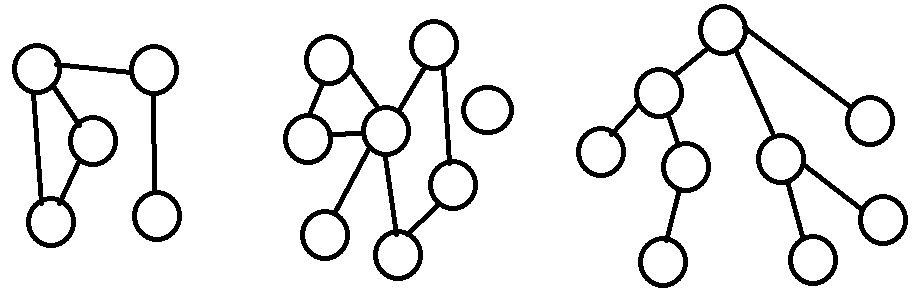
\includegraphics[scale = .45]{imagens/grafos.png}}
       \label{fig:grafos}
    \fonte{Elaboração Própria}
\end{figure}
\end{frame}


\begin{frame}
    \begin{teo}
$G$ é uma árvore se, e somente se, é conexo e acíclico.
\end{teo}
\end{frame}



\begin{frame}


\begin{itemize}
    \item Fazemos uma série de perguntas verdadeiro/falso em sequência 
    \\
    \\
    e.g. Um cliente tem mais de $x$ anos de idade, compra mais de $y$ reais por mês, um tomador de crédito tem menos de $z\%$ de alavancagem etc
    \item Representamos isso como uma série de bifurcações partindo de uma origem, graficamente temos uma \textbf{árvore}

\end{itemize}
\end{frame}


\begin{frame}

\begin{figure}[H]
    \centering
    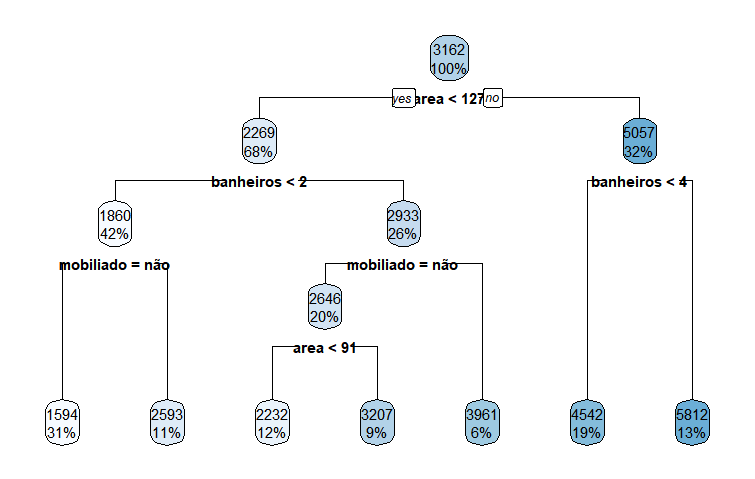
\includegraphics[scale = .55]{imagens/arvore_decisao_houses.png}
    \caption{Um exemplo de árvore de regressão.}
    \label{fig:arvore_reg}
\end{figure}
\end{frame}




\begin{frame}
Surge uma questao: como escolher testes, em qual ordem e com quais parametros? Escolha a pergunta cuja resposta maximiza alguma métrica de qualidade.

\begin{itemize}
    \item \textbf{Classificação:} Impureza de Gini entre classes, Ganho de Informação 
    \item \textbf{Regressão:} Diferença de média entre grupos, soma ponderada das variâncias da variável resposta em cada nodo filho
\end{itemize}

Basta repetir o processo da partilha até que algum dos nodos filhos tenha menos observações do que uma amostra mínima, ou nenhuma partição tenha um valor mínimo para a métrica de qualidade.


\end{frame}

\begin{frame}
\begin{itemize}
    \item \textbf{Nenhum teste cumpre um valor mínimo para a métrica de qualidade} \newline Cada pergunta respondida diminui a informação disponível, tornando o ganho de informação cada vez menor. Alguma hora, a cargo do modelador definir, uma pergunta adicional provavelmente custa mais em parcimônia e computação do que devolve em acurácia de previsão. É hora de gerar uma folha.
    
    \item \textbf{O número de perguntas feitas chegou ao máximo} \newline
    Uma maneira de forçar parcimônia do modelo é limitar o número de perguntas. Algumas implementações diferenciam o número total de perguntas do número de perguntas sucessivas.  
\end{itemize}
    
\end{frame}

\begin{frame} 
\begin{itemize}
   \item \textbf{O número de observações do nodo não cumpre um mínimo} \newline 
 
    A amostra que chegou no nodo está abaixo de um mínimo. Por ser um dos mais simples e ter uma relação diretamente proporcional com o número de regras de previsão/classificação distintos é um dos mais comuns na literatura.
\end{itemize}
    
\end{frame}

\begin{frame}

\textbf{Ganho de Informação}:

\begin{align}
    H(n_i) = - \sum_{p_j \in P(n_i)} p_j \log_2 p_j, 
\end{align}

\begin{align}
    \I_E(\tau) = H(n_i) - P(a\, |\, \tau) \,H(n_i \, |\,  a) - P(b \,| \,\tau)\, H(n_i \, |\,  b)
\end{align}

Escolhemos, dentro do conjunto de testes $\mathcal{T}$:

\begin{align}
    \tau^*(n_i) = \underset{\tau \in \mathcal{T}}{\text{arg max}} \, \, \I_E(\tau)
\end{align}


\textbf{Impureza de Gini}:
 
 \begin{align}
     G(n_i) = \sum_{i = 1}^J p_i ( 1  - p_i) =  1 - \sum_{i = 1}^J p_i^2
 \end{align}


\end{frame}

% FALAR DOS GATILHOS DE TRAVA AQUI

\begin{frame}
\textbf{Problema:} árvores de decisão performam bem com poucas classes e muito mal em regressão. A variância cresce não-linearmente no número de regras de classificação. 


\begin{figure}[H]
    \centering
    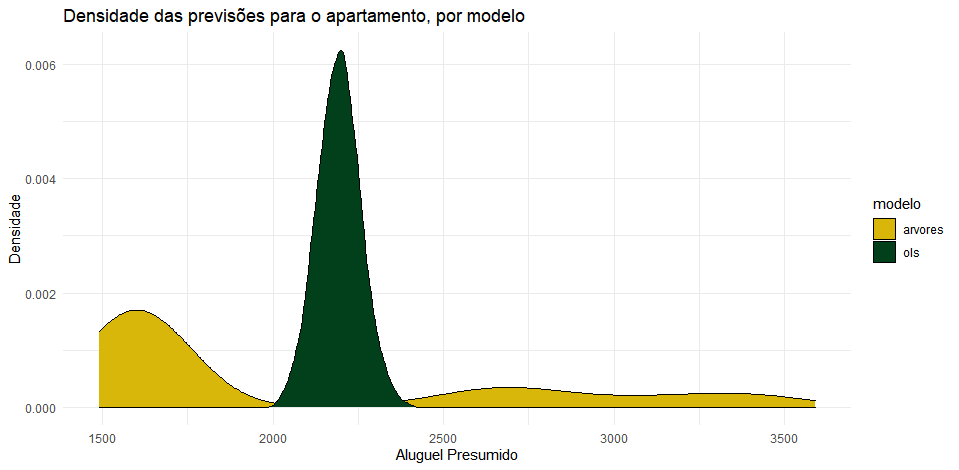
\includegraphics[scale = .40]{imagens/exemplo_var_arvores.png}
    \caption{A distribuição das previsões por classe de modelo.}
    \label{fig:arvore_var_ols}
\end{figure}
\end{frame}


\begin{frame}
Como lidar com isso? Uma maneira de mitigar a variância é treinar não só uma, mas várias árvores e usar a média de suas previsões como previsão final. Como árvores têm variância finita, a média da floresta tem distribuição normal e variância finita.

\begin{teo}[Lindenberg-Lévy]
Seja $(\textbf{X}_1, ..., \textbf{X}_n)$ uma amostra independente e identicamente distribuída com $\E[\textbf{X}_i] = \mu$ e $\V[\textbf{X}_i] = \sigma^2 < \infty$. Então:

\begin{align}
    \sqrt{n}\,(\bar{\textbf{X}_i }- \mu) \xrightarrow[n \to \infty]{d} N(0, \sigma^2)
\end{align}

\end{teo}
\end{frame}


\begin{frame}
Maneiras de mitigar a variância da floresta:

\begin{itemize}
    \item Treinar árvores \textit{rasas}, com poucas regras de classificação, portanto com menos variância
    \item Expor as árvores a subconjuntos dos dados (\textbf{bagging}, na literatura)
    \item Expor as árvores a um subconjunto das variáveis explicativas
\end{itemize}
\end{frame}



\begin{frame}
O que ainda não temos? Interpretabilidade. O modelo não entrega os efeitos marginais como em modelos lineares.

\begin{align}
    \hat{y}_i = \beta_0 + \sum_{j=1}^{k} \beta_j \mathbf{x}_{ij} 
\end{align}


\begin{align}
    \frac{\partial \hat{y}_i}{\partial \mathbf{x}_{ij} } = \beta_j
\end{align}
\end{frame}

\begin{frame}

A forma funcional de uma árvore de decisão é de pouco interesse. Tendo uma regra de previsão $\hat{y}_i$ para cada grupo possivel de $k$ opções:

\[
    \hat{y}(\mathbf{x}) = \left.
    \begin{cases}
    \hat{y}_1  ,\,\mathbf{x} \in \text{Grupo 1} \\
    \hat{y}_2  , \,\mathbf{x} \in \text{Grupo 2} \\
    ...\\
    \hat{y}_k  ,\, \mathbf{x} \in \text{Grupo $k$}\\
    \end{cases}
    
\]
   
\end{frame}


\begin{frame}

\textbf{Desejo:} Ter uma curva que em caso de um processo verdadeiramente linear seja constante no mesmo nível de $\beta_j$ e, caso não, aproxime o efeito marginal localmente.
\newline

\textbf{Proposta:} Simular uma observação de referência e uma grade de observações ao seu redor para computar as previsões de uma floresta treinada nessa grade.


\end{frame}

\begin{frame}
Em um experimento controlado onde sabemos que os efeitos marginais são constantes, o que acontece?

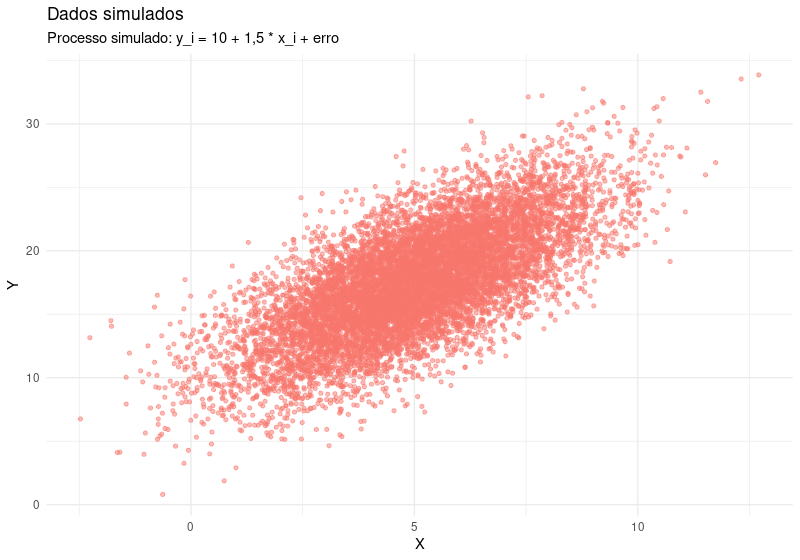
\includegraphics[scale = .50]{imagens/exemplo_freddy_fake_data.png}
    
\end{frame}


\begin{frame}
    \begin{figure}[H]
    \centering
    
    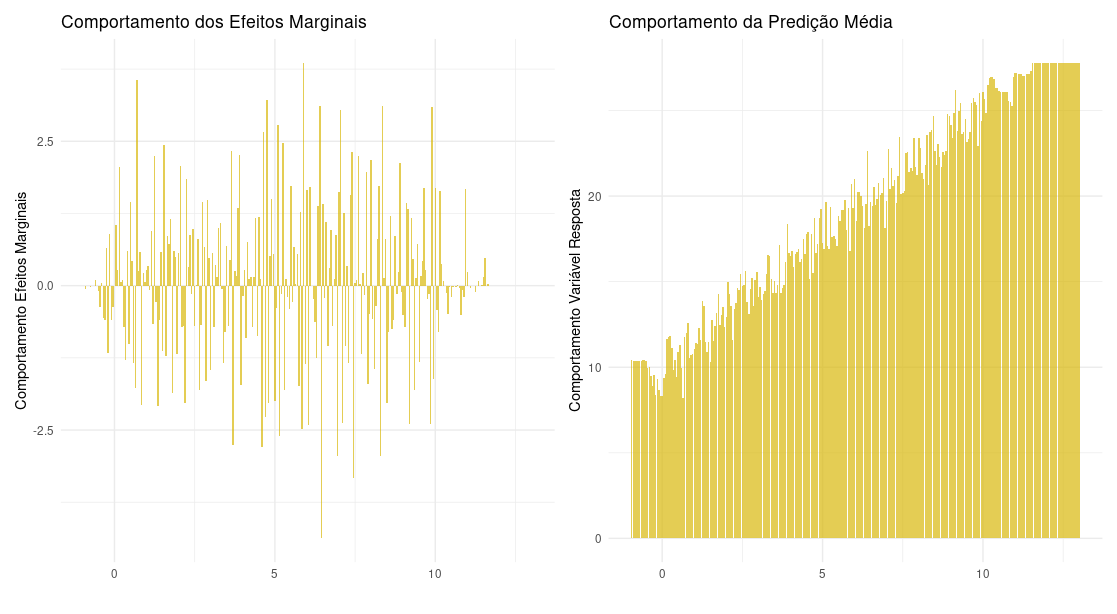
\includegraphics[scale = .35]{imagens/exemplo_freddy_efeitos_marginais.png}

\end{figure}

\end{frame}






\begin{frame}
E em um ambiente não-controlado? 

\end{frame}

\begin{frame}
    \begin{itemize}
    \item \textbf{Razão Performance-Interquatil (RPIQ)} \newline
    Definida como o desvio-padrão das previsões dividido pela amplitude interquartil observada da resposta.
    
    \item \textbf{Coeficiente de Concordância de Correlação (CCC)} \newline
    Diferença entre a identidade e a reta de regressão dos valores preditos nos observados. 
    
    \item \textbf{Erro Médio Absoluto (MAE)} \newline
    A média das diferenças entre previsões e valores observados. 
    

\end{itemize}
\end{frame}

\begin{frame}

\begin{itemize} 
    \item \textbf{Erro Médio Percentual (MPE)} \newline
    A média das diferenças entre previsões e valores observados ponderada pela média da resposta.
    
    \item \textbf{Coeficiente de Determinação (R2)} \newline
    Quadrado da correlação entre valores preditos e observados.
    
    \item \textbf{Raiz do Erro Quadrático Médio (RMSE)} \newline
    Raiz da média dos quadrados dos desvios das previsões em relação aos valores observados.
    
\end{itemize}
\end{frame}


\begin{frame}
\begin{itemize}
    \item \textbf{Sensitividade/ Recall} \newline
    Em classificação binária, a Sensitividade é a proporção dos casos positivos que são corretamente identificados.
    \item \textbf{Especificidade} \newline
    Em classificação binária, a Especificidade é a proporção dos casos negativos que são corretamente identificados.
    \item \textbf{Acurácia} \newline
    A fração de casos corretamente identificados. 
    \item \textbf{Precisão/ Valor Preditivo Positivo} \newline
    O número de observados positivos dividido pelo número de preditos positivos.
    \item \textbf{F1-Score} \newline
    Média harmônia da Precisão e da Sensitividade
\end{itemize}
    
\end{frame}

\begin{frame}
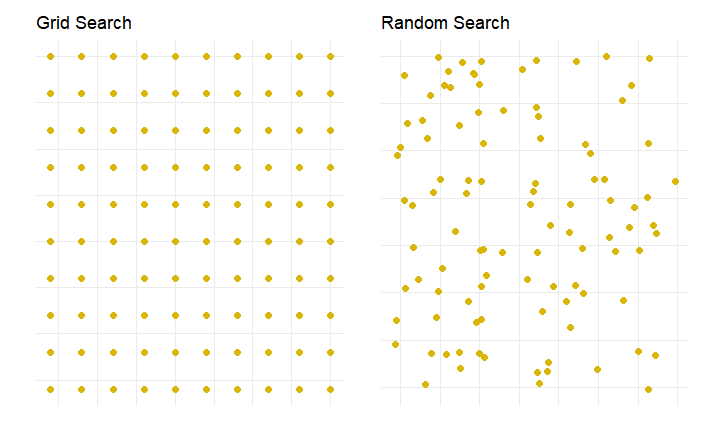
\includegraphics[scale = .60]{imagens/random_grid.png}
    
\end{frame}


\begin{frame}

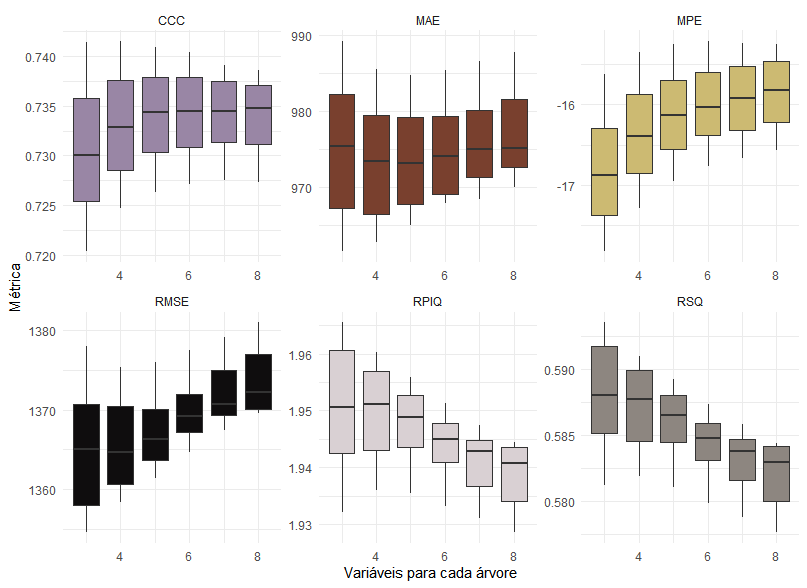
\includegraphics[scale = .50]{imagens/cross_v_mtry.png}
    
\end{frame}


\begin{frame}

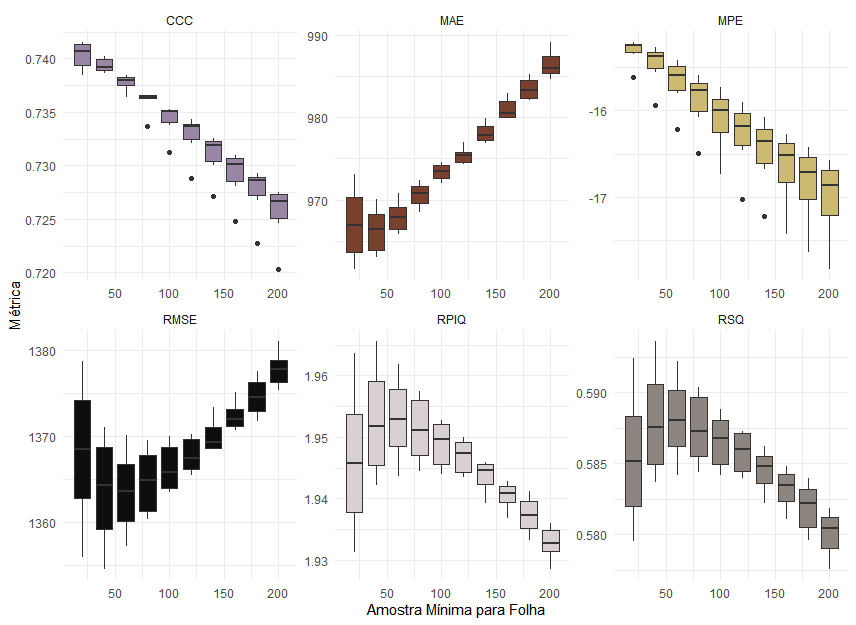
\includegraphics[scale = .45]{imagens/crossv_min.png}
    
\end{frame}


\begin{frame}

\begin{figure}[H]
    \label{ols_marg}
    \centering
    
    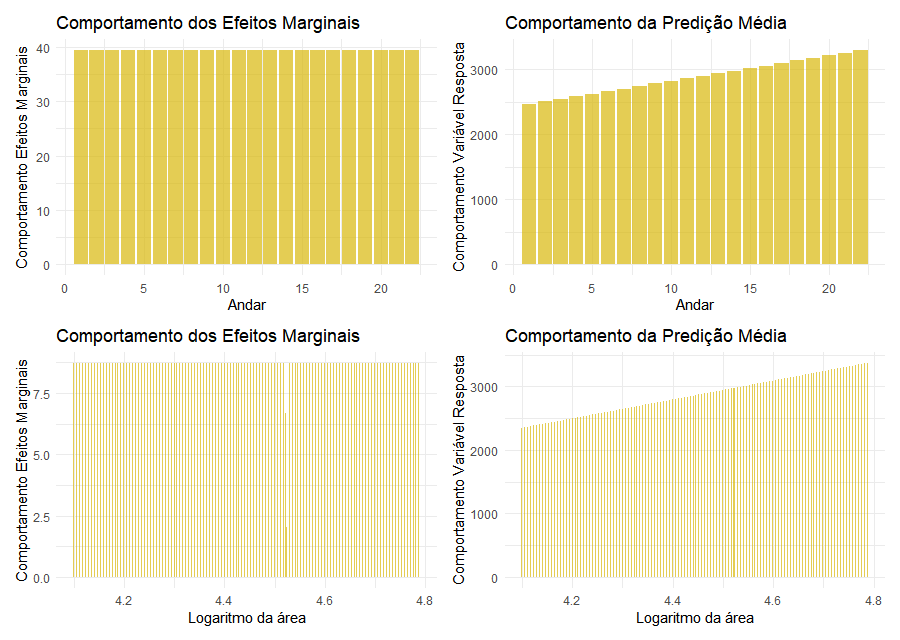
\includegraphics[scale = .45]{imagens/efeitos_marginais_lm.png}
\end{figure}

\end{frame}

\begin{frame}
\begin{figure}[H]
    \centering
    
  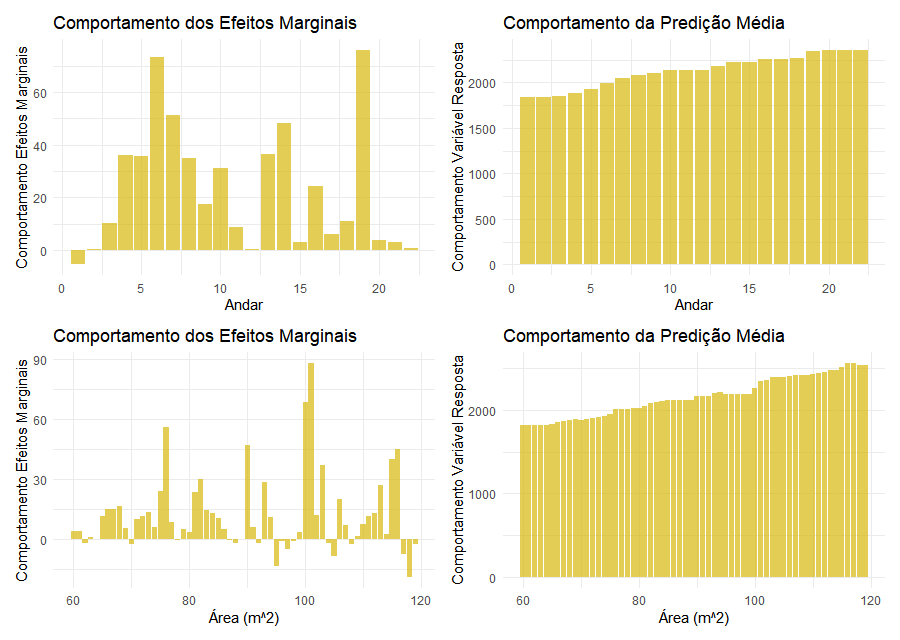
\includegraphics[scale = .45]{imagens/efeitos_marginais_RF.png}
\end{figure}
\end{frame}


\bibliography{referencias.bib}








\end{document}